%%%%
\documentclass[10pt]{report}
\usepackage{graphicx,color,epsfig,psfig,subfigure}
\usepackage{amsmath,amsfonts,amssymb}
\usepackage{bm}
\pagestyle{empty}
\begin{document}
\begin{picture}(0,0)%
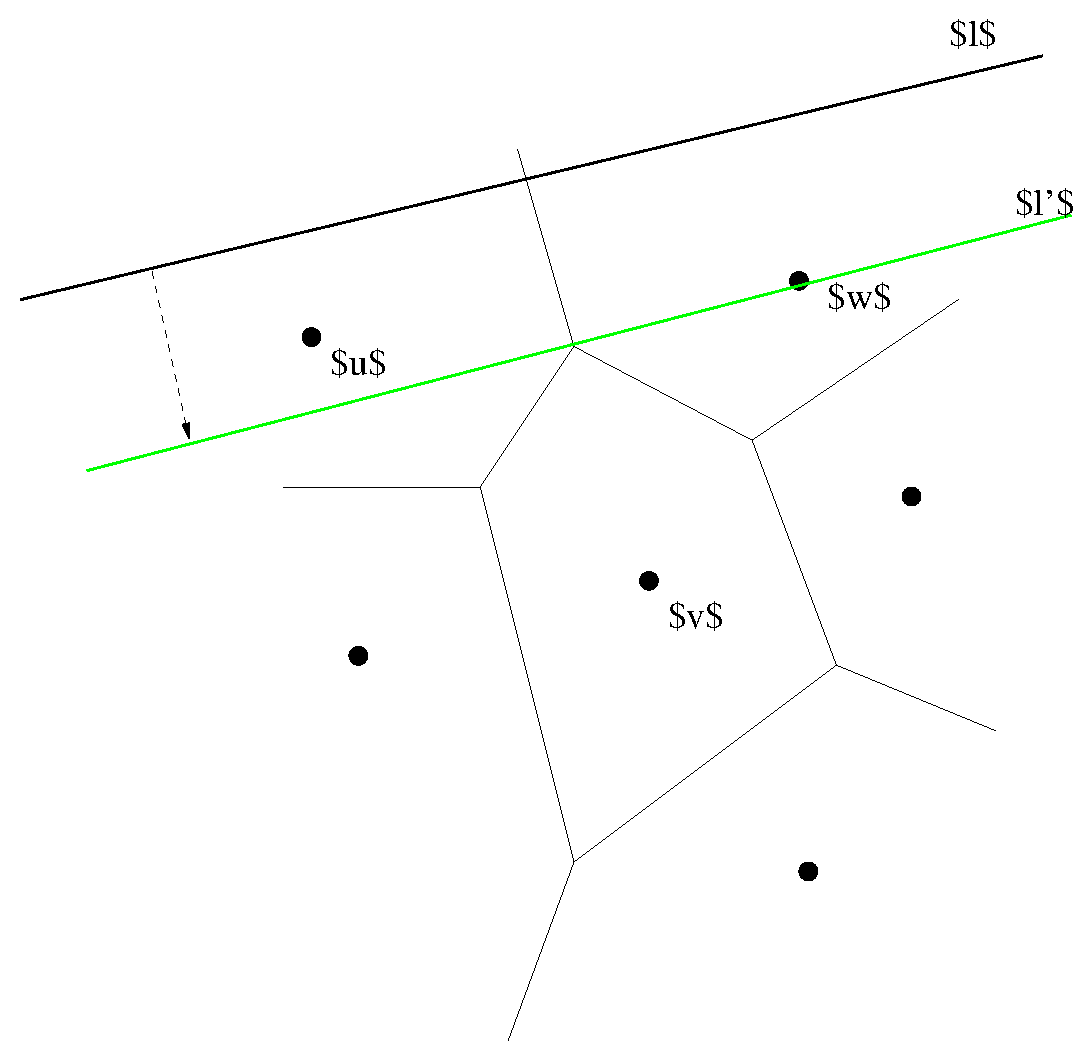
\includegraphics{preuve_cache.pstex}%
\end{picture}%
\setlength{\unitlength}{3947sp}%
%
\begingroup\makeatletter\ifx\SetFigFont\undefined%
\gdef\SetFigFont#1#2#3#4#5{%
  \reset@font\fontsize{#1}{#2pt}%
  \fontfamily{#3}\fontseries{#4}\fontshape{#5}%
  \selectfont}%
\fi\endgroup%
\begin{picture}(8444,8202)(579,-8098)
\put(5776,-4786){\makebox(0,0)[lb]{\smash{\SetFigFont{20}{24.0}{\familydefault}{\mddefault}{\updefault}{\color[rgb]{0,0,0}$v$}%
}}}
\put(7051,-2236){\makebox(0,0)[lb]{\smash{\SetFigFont{20}{24.0}{\familydefault}{\mddefault}{\updefault}{\color[rgb]{0,0,0}$w$}%
}}}
\put(8551,-1486){\makebox(0,0)[lb]{\smash{\SetFigFont{20}{24.0}{\familydefault}{\mddefault}{\updefault}{\color[rgb]{0,0,0}$l'$}%
}}}
\put(8026,-136){\makebox(0,0)[lb]{\smash{\SetFigFont{20}{24.0}{\familydefault}{\mddefault}{\updefault}{\color[rgb]{0,0,0}$l$}%
}}}
\put(3076,-2761){\makebox(0,0)[lb]{\smash{\SetFigFont{20}{24.0}{\familydefault}{\mddefault}{\updefault}{\color[rgb]{0,0,0}$u$}%
}}}
\end{picture}
\end{document}
